
\section{Building StanfordExtra: a new large-scale dog keypoint dataset}

\begin{figure*}[h]
    \centering
    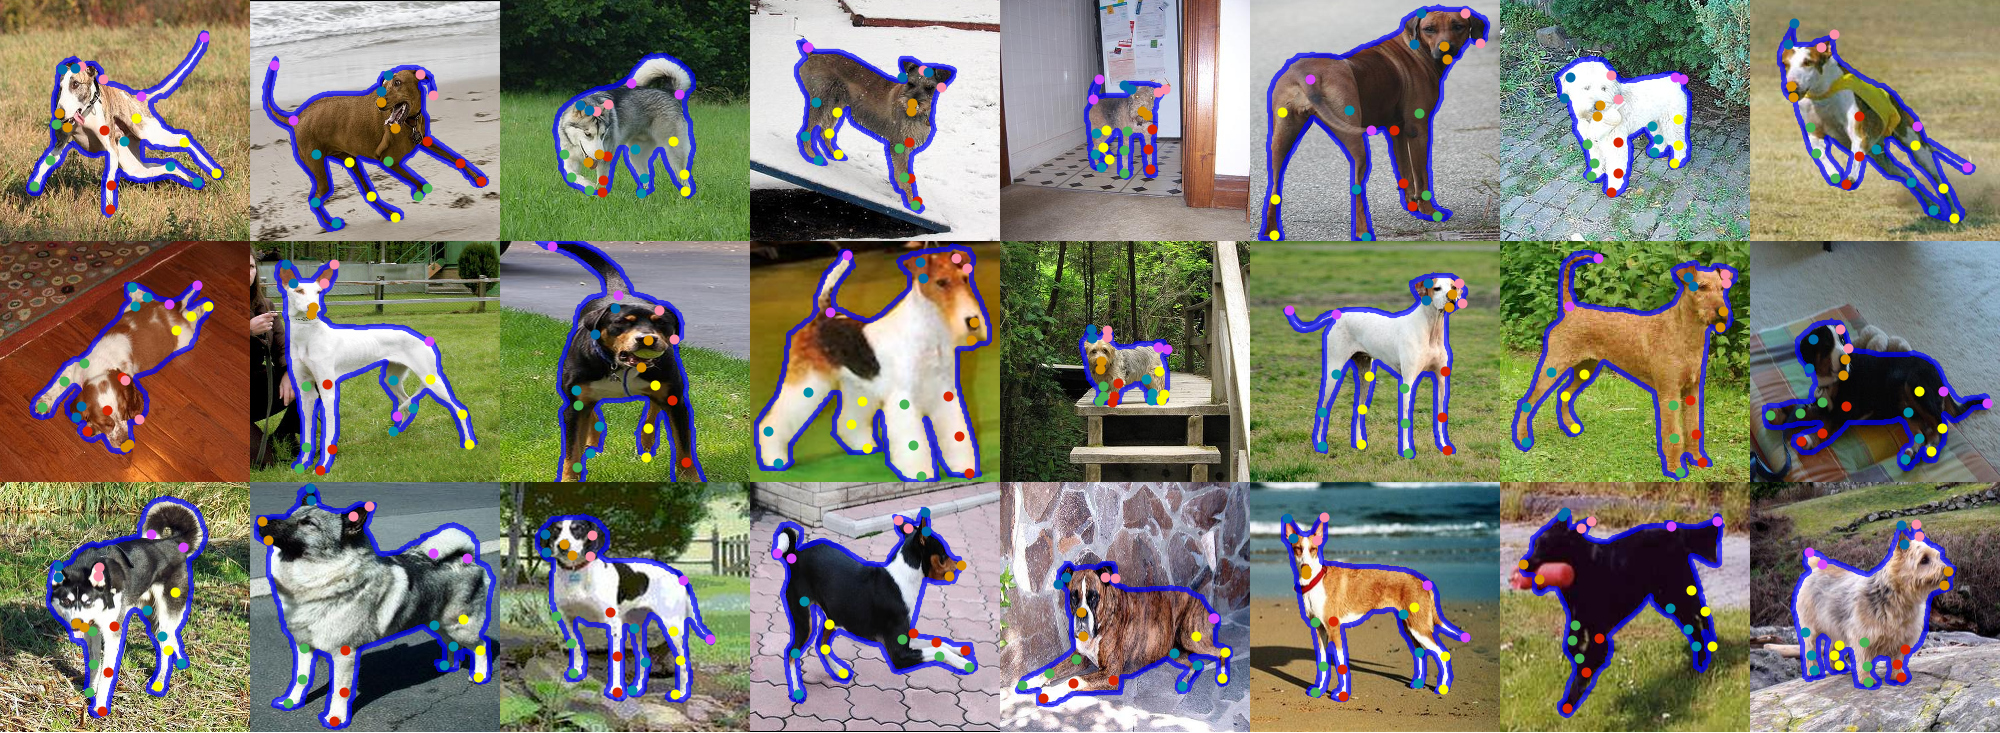
\includegraphics[height=0.1775\textheight]{OllieFigs/collage_wide.png}
    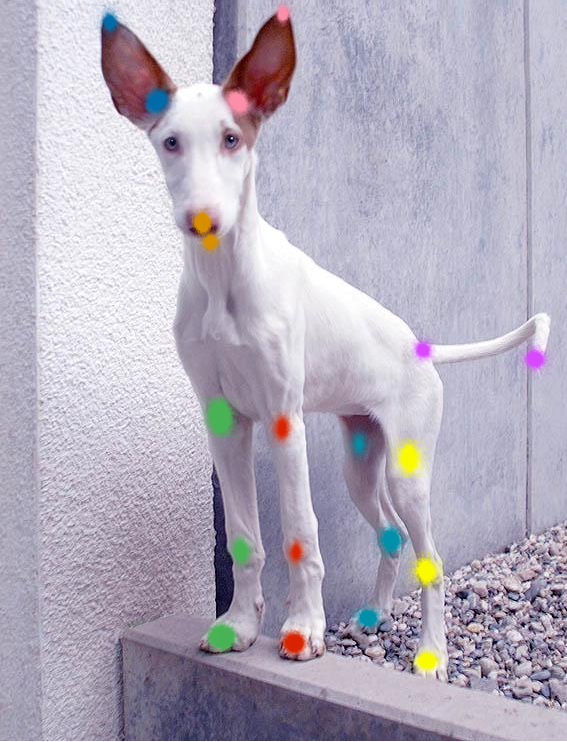
\includegraphics[height=0.1775\textheight]{OllieFigs/heatmap.png}
    \caption{\textbf{StanfordExtra example images}. \emph{Left}: outlined segmentations and labelled keypoints for 24 representative images. \emph{Right}: heatmap of deviation of worker submitted results from mean for each submission.}
    \label{fig:dataset}
\end{figure*}

In order to evaluate our method, we introduce \emph{StanfordExtra}: a new large-scale dataset with annotated 2D keypoints and binary segmentation masks for dogs. We opted to take source images from the existing Stanford Dog Dataset~\cite{StanfordDogs}, which consists of 20,580 dog images taken ``in the wild" and covers 120 dog breeds. The dataset contains vast shape and pose variation between dogs, as well as nuisance factors such as self/environmental occlusion, interaction with humans/other animals and partial views. Figure~\ref{fig:dataset} (left) shows samples from the new dataset.

We used Amazon Mechanical Turk to collect a binary silhouette mask and 20 keypoints per image: 3 per leg (knee, ankle, toe), 2 per ear (base, tip), 2 per tail (base, tip), 2 per face (nose and jaw). We can approximate the difficulty of the dataset by analysing the variance between 3 annotators at both the joint labelling and silhouette task. Figure~\ref{fig:dataset} (right) illustrates typical per-joint variance in joint labelling. Further details of the data curation procedure are left to the supplementary materials. 


In this section, we describe our process for  obtaining keypoint and segmentation annotations for the Stanford Dog Dataset~\cite{StanfordDogs}. We submit the entire set of 20,580 dog images to the Amazon Mechnical Turk crowdsourcing platform to obtain a set of 20 keypoint and segmentation masks. We overlay 1 bounding box, provided with the original dataset, on the submitted images to identify the specific dog for the annotators to label. Each image was sent to 3 independent annotators for collecting keypoints and segmentation masks.

\subsection{Keypoints.} 
To identify keypoints, workers were given a list of 20 keypoints to click: 2 per tail, 3 per leg, 2 per ear, nose and jaw. They were additionally asked to provide a visibility flag per point. 

For each keypoint, we process the three clicks to yield a reliable coordinate. From the 3 clicks, we discard clicks that are further than a set tolerance from the mean. If at least 2 clicks remain, we take the mean coordinate as the accepted keypoint position. Otherwise, the point has not been reliably identified between workers, so we set the keypoint as invisible. As described in the main paper, we remove images from train and test splits which have fewer than 8 visible keypoints.

% We rely on the following scheme to determine the optimal position of each keypoint, from the three annotations:

% \begin{enumerate}
%     \item 
% \end{enumerate}

% \begin{enumerate}
% \itemsep0em 
% \item{If If the keypoint was flagged highlighted by three different workers, and all three points are within a certain tolerance of the mean\footnote{Tolerance set at (Image width + Image height)/80, in pixels.}, then accept the mean as the keypoint position. If not, reject the furthest point from the mean, and go to step 2.}

% \item{If the keypoint was highlighted by two different workers, and both points are within a certain tolerance of the mean, accept the mean as the keypoint position. If not, reject the keypoint.}

% \item{If the keypoint was highlighted by only one worker, reject the keypoint.}

% \end{enumerate}


\subsection{Segmentation.}

For each image, each worker $w \in \{w_{1}, w_{2}, w_{3}\}$ submits a binary segmentation mask $\mathbf{A}^{w} \in \mathbb{R}^{H \times W}$. We request a re-labelling for any submissions which fail simple criteria, such as if the highlighted area is below a threshold number of pixels.

% In order to sanitise the dataset and reduce erroneous entries, certain images were rejected or discarded. `Discarded' refers to a submission being discarded from the final dataset, whilst `rejected' means that the submission was deleted from the MTurk dataset, and a new entry requested from the website.\\

% As an initial pass, images were rejected (for which the bounding boxes were insufficiently large - to count null entries. For this, any entry was rejected if,

% \begin{equation}
% \sum\limits_{j=1}^H \sum\limits_{k=1}^W \mathbf{A}^{i,w}_{jk} < 0.01 WH 
% \end{equation}

For each image, we generate the most likely segmentation by comparing submissions across workers. For any two workers $w, w'$ we compute a correlation coefficient:

\begin{equation}
c_{w,w'} = \frac{\sum_i\sum_j \left[ \mathbf{A}^{w} \odot \mathbf{A}^{w'} \right]_{i,j}}{\max\limits_{p = \{w,w'\}} \sum_{i} \sum_{j} \mathbf{A}^p_{i,j}}
\end{equation}

% \begin{equation}
% c_{w,w'} = \frac{\mathbf{A}_{w} \odot \mathbf{A}_{w'}}{\max\limits_{p = \{w, w'\}}\mathbf{A}_{p}}
% \end{equation}

% We remove annotations for which all correlation coefficients are below 80\%. 
Where $\odot$ denotes the element-wise product of the matrices. We remove a worker's segmentation $A^{w}$ if all correlation coefficients $c_{w,w'}$ are below a set threshold. The final binary mask is computed from the remaining submissions:

\begin{equation}
\hat{A}_{i,j} = \begin{cases}
    1, & \text{if } \sum_w A^{w}_{i,j} > 1 \\
    0,              & \text{otherwise}
\end{cases}
\end{equation}

\begin{figure}
\centering
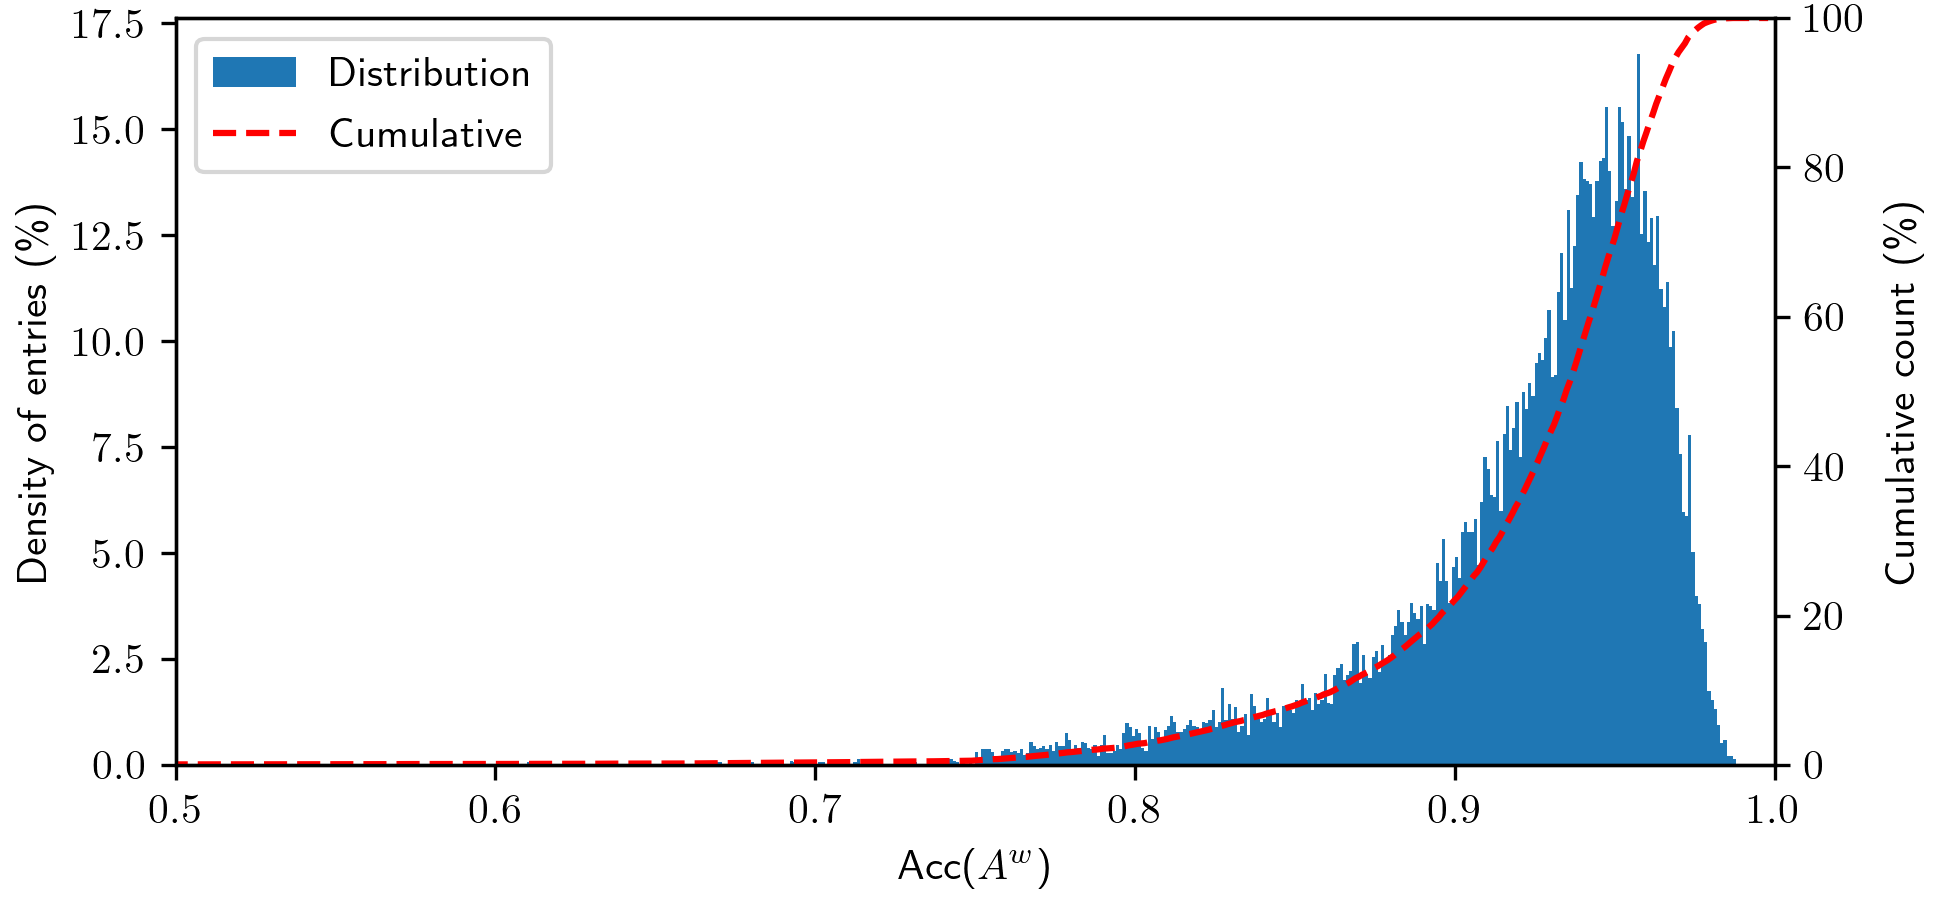
\includegraphics[width=0.95\textwidth]{OllieFigs/correlations.PNG}
\caption{Accuracy distribution of all submitted dog segmentations across the entire Stanford Dog Dataset.}
\label{fig:accuracy distribution}
\end{figure}

We can also define the accuracy of a worker's segmentation, as the largest of their correlation coefficients: $\textrm{Acc}(A^{w})=\max_{w'\neq w} \{c_{w,w'}\}$. Figure \ref{fig:accuracy distribution} shows the set of segmentation annotation accuracies over the entire labelled dataset.

% \subsubsection{Filtering the dataset.}

% As described in the paper, we reject images from our train/evaluation splits which based on reliability we deem unsuitable for our task of complete 3D reconstruction. have fewer than 8 identified keypoints find it necessary to reject The Stanford dog dataset contains 20,580 images. Not all of these images are constructive to this dataset - many do not have a lot of the dog in frame, etc. Several stages of refinement of the dataset were made, detailed in Table \ref{tab:filtering}.

% \begin{table}[]
%     \centering
%     \begin{tabular}{c|c}
%          \toprule
%          20,580 &  Stanford dataset\\
%          - (5,...) & Initial filtering based on bbox \\
%          - (5,...) & Images with fewer than 8 identified keypoints \\
%          - (60) & Images with insufficient segmentation accuracy \\
%          - (76) & Images for which more than one keypoint is outside of the segmentation\footnote{(with padding of 5 pixels)}\\
%          \midrule
%          9,647 & Final dataset\\
%          \bottomrule
%     \end{tabular}
%     \caption{Filtering process for final produced dataset}
%     \label{tab:filtering}
% \end{table}
